% Documento pronto da stampare
\documentclass[a4paper,12pt,oneside]{report}


\usepackage{xcolor}
% Imposto la lingua italiana
\usepackage[italian]{babel}


% Settaggio dei margini 
\topmargin 0cm 
\headsep 1cm 
\headheight 0.6cm
\textwidth 14.6cm
\textheight 21.8cm
\evensidemargin 1cm 
\oddsidemargin 1cm
% 				VEDERE COME METTERE INTERLINEA!!!!  \linespread{1.1}
% Pacchetti da includere per...

\newtheorem{theorem}{Teorema}[section]  % sec. number + seq. number
\newtheorem{definition}[theorem]{Definizione}
\newtheorem{lemma}[theorem]{Lemma}
\newtheorem{corollary}[theorem]{Corollario}
\newtheorem{proposition}[theorem]{Proposizione}
\newtheorem{remark}[theorem]{Osservazione}
\newtheorem{example}[theorem]{Esempio}
\renewcommand{\labelenumi}{(\alph{enumi})}
 

\usepackage{amsthm}

% simboli matematici
\usepackage{amsmath} 
\usepackage{amssymb} 
\usepackage{amsfonts} 
\usepackage{bbm} 
% simboli vari
\usepackage{textcomp}                      
\usepackage[mathscr]{euscript}

% figure 
\usepackage{epsfig}
\usepackage{graphicx}
\usepackage{subfigure}


% intestazioni
\usepackage{fancyhdr}

% encoding dei caratteri
\usepackage[ansinew]{inputenc}
\usepackage[OT1]{fontenc}

% riferimenti cliccabili nel pdf
\usepackage[pdftex]{hyperref} 

\usepackage{array}

% Stile della pagina
\fancyhead[L]{\chaptername \thechapter}
\fancyhead[LO]{\thesection} \fancyhead[RO]{\sectionmark}
\lhead{\slshape Ch. \thechapter}

% Configurazioni varie

% nonumchapter serve per introduzioni, prefazioni, ecc.
% titola come un capitolo ma senza numero
\def\nonumchapter#1{
	\chapter*{#1}
	\addcontentsline{toc}{chapter}{#1}
}

% estensioni e cartella delle immagini (non necessario...)
\DeclareGraphicsExtensions{gif,eps,png,jpeg}
\graphicspath{{./eps/}}

% crea una nuova lunghezza e gli assegna un valore
\newlength{\defbaselineskip}
\setlength{\defbaselineskip}{\baselineskip}

% comando per settare  la variabile \baselineskip come multiplo di \defbaselineskip
\newcommand{\setlinespacing}[1]%
           {\setlength{\baselineskip}{#1 \defbaselineskip}}

% permette l'inserimento "rapido" del virgolettato (ad es. per citazioni)
\newcommand{\virgolette}[1]{``#1''}

% Settaggio interlinea 
\setlinespacing{1.5}


% Impostazioni della pagina
\usepackage{indentfirst}
\cfoot{\thepage}


%opening


\begin{document}
\pagenumbering{arabic}
%%%%%%%%%%%%%%%%%%%%%%%%%%%%%%%%%%%%%%%%%%%%%%%%%%%%%%%%%%%%%%%%%%%%%
%                                                                   %
%                           TESI in LaTex                           %
%                                                                   %
%%%%%%%%%%%%%%%%%%%%%%%%%%%%%%%%%%%%%%%%%%%%%%%%%%%%%%%%%%%%%%%%%%%%%


%%%%%%%%%%%%%%%%%%%%%%%%%%%%%%%%%%%%%%%%%%%%%%%%%%%%%%%%%%%%%%%%%%%%%
%                         Inizio Documento                          %
%%%%%%%%%%%%%%%%%%%%%%%%%%%%%%%%%%%%%%%%%%%%%%%%%%%%%%%%%%%%%%%%%%%%%



\thispagestyle{empty}
\enlargethispage{60mm}
\begin{titlepage}
\begin{center}
\textsc{ \LARGE{U}\LARGE{niversit\`a}\ \LARGE{degli}\
\LARGE{S}\LARGE{tudi}\ \LARGE{di}\
\LARGE{G}\LARGE{enova}\\
\vspace{0.3cm}

\includegraphics[scale=0.2]{unige.PNG}\\
\vspace{0.5cm}
{\LARGE Facolt\`a di Scienze Matematiche, Fisiche e Naturali}}\\
\vspace{5mm}
\Large Corso di studi in \\
\large Statistica Matematica e trattamento Informatico dei Dati\\
\vspace{0.5cm}

\includegraphics[scale=0.6]{smid.PNG}\\
\vspace{0.5cm}
\Large Anno accademico 2013/2014\\
\vspace{0.7cm}
{\LARGE Tesi di Laurea}\\
\vspace{0.70cm}
\begin{LARGE}
\textbf{Metodi di Adaboost Multiclasse}\\
\end{LARGE}
\vskip 1.2cm

\begin{LARGE}

\textbf{Candidato:}\\
D'Angelo Giacomo

\vskip 1.5cm
\centering
\parbox{17cm}{
    \hspace{1cm} \textbf{Relatore:} \hspace{4.3cm} \textbf{Correlatore:} \\  
    Dott. Fabrizio Malfanti  \hspace{1.2cm} Prof.ssa Eva Riccomagno
 }


\end{LARGE}
\end{center}
\end{titlepage}

\newpage
\vspace{2.0cm}
\begin{flushright}
 \begin{it}
 ``Sky's the limit''
 \end{it}\\
The notorious B.I.G.
\end{flushright}



\tableofcontents
\chapter{Introduzione}
\ \
\newline
La tesi di laurea riguarda l'approfondimento
delle teorie inerenti al mondo degli algoritmi di boosting: i procedimenti, le peculiarit\`a e le differenze 
di utilizzo per le principali versioni di Adaboost, avendo io 
avuto un primo approccio durante lo 
svolgimento del tirocinio relativo a questi algoritmi.\\
\section{Obiettivo}
Obiettivo di questa tesi \`e mostrare l'algoritmo adaboost nella sua versione multi-classe e alcune varianti 
ed estensioni; infatti esistono diverse versioni per affrontare il problema multivariato 
ognuna delle quali differisce per una qualche caratteristica che verr\`a analizzata nei prossimi paragrafi.\\
Lo scopo del tirocinio svolto \`e stato quello di costruire un filtro Adaboost per la classificazione di previsioni sportive, in modo tale da
ottenere un classificatore che risulti pi\`u efficace rispetto a quelli 
utilizzati per la costruzione del filtro; ovvero attraverso questo algoritmo si 
vuole combinare un numero finito di bookmakers per la costruzione di uno virtuale.
Questo bookmaker virtuale si pone come obiettivo quello di predire correttamente l'esito di pi\`u 
partite rispetto ai bookmakers utilizzati per costruire il filtro.\\
Lo studio effettuato nella tesi \`e servito per capire se l'algoritmo Adaboost fosse realmente quello migliore, 
rispetto a tutti gli altri algoritmi, per
il problema preso in considerazione. Si sono quindi analizzati a fondo le caratteristiche dell'Adaboost per 
verificare se quello scelto inizialmente fosse realmente la versione pi\`u efficiente per 
la risoluzione del problema riscontrato durante il tirocinio. 


\newpage
\vspace{1.5cm}

\section{I dati}
Il dataset considerato si riferisce agli ultimi cinque anni di previsioni sportive 
inerenti al campionato di calcio tedesco,
la Bundesliga e a quello inglese, la Premier League.\\
\newline
I dati sono stati reperiti sul sito  \begin{it}Football-data.uk\end{it}, il quale riporta per ogni anno:
\begin{itemize}
 \item DATA: data in cui \`e stata giocata la partita
 \item HOME\_TEAM: nome squadra che gioca in casa
 \item AWAY\_TEAM: nome squadra che gioca in trasferta
 \item RESULT: esito reale della partita
 \item QUOTAS\_H: previsione dell'esito vittoria in casa
 \item QUOTAS\_D: previsione dell'esito pareggio
 \item QUOTAS\_A: previsione dell'esito vittoria in trasferta
\end{itemize}
 Le tre quote sono prese per cinque bookmakers:
\begin{itemize}
 \item BW: Bet\&Win
 \item IW: Interwitten
 \item LB: Ladbrokes
 \item SJ: StanJames
 \item WH: WilliamHill
\end{itemize}
\newpage
\vspace{1.5cm}
I file a disposizione per il progetto erano nella forma rappresentata in Figura~1.1\\
\vspace{1.5cm}
\begin{figure}
 \makebox[\textwidth][c] {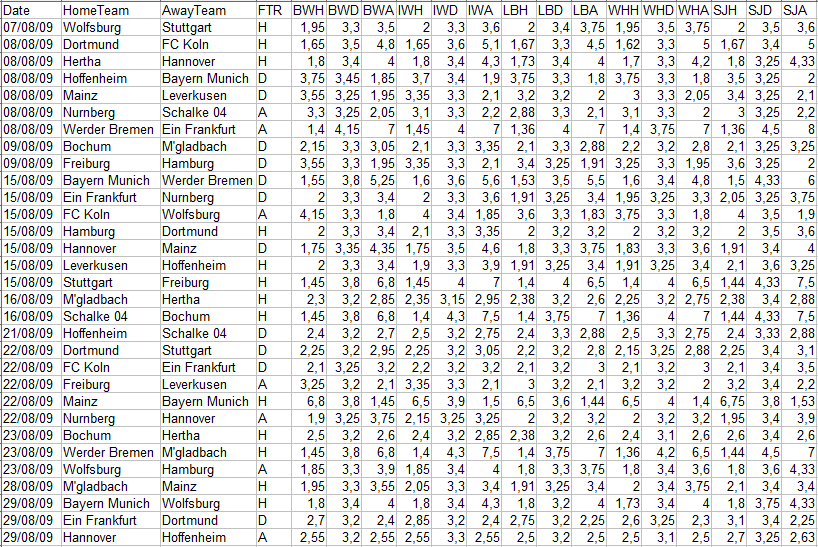
\includegraphics[width=1.3\textwidth]{dati.png}}
 \caption{Esempio file di dati a disposizione}
 \label{fig:dati}
\end{figure}


\newpage
\vspace{1.5cm}
\section{Data description}
Studiare i dati che avevamo a disposizione ha portato a capire come sia vasta la casistica nel mondo dei 
filtri di boosting. Per una migliore comprensione introduciamo i termini ``due/multi-classe'', ovvero gli 
stati d'uscita dell'evento, che possono essere di tipo dicotomico o multinomiale e 
``single/multi-label'', ovvero la classificazione del 
determinato evento, che pu\`o essere sempre la stessa o variare. Quest'ultimo concetto 
\`e spiegato graficamente attraverso la tabella seguente:\\
\newline
\begin{table}[!h]
\centering
\begin{tabular}{|c|c|c|}
\hline
Squadra A&Squadra B&Esito\\
\hline
Juventus&Chievo&1\\
\hline
Juventus&Chievo&1\\
\hline
Juventus&Chievo&1\\
\hline
Juventus&Chievo&1\\
\hline
Juventus&Chievo&X\\
\hline
\end{tabular}
\end{table}
\ \
\newline
L'oggetto partita Juventus-Chievo, ogni volta che sar\`a giocata, avr\`a la 
possibilit\`a di essere classificata in maniera diversa, e quindi potr\`a assumere 
pi\`u di un tipo di label.
Ogni combinazione ``due/multi-classi'' con ``single/multi-label'' viene affrontata da 
una versione dell'algoritmo, come vedremo
nei prossimi capitoli. \\
\newline
\begin{table}[!h]
\centering
\begin{tabular}{|c|c|c|}
\hline
Versione&Classe&Label\\
\hline
Alga Tossica&Due-Classi&Single-label\\
\hline
\end{tabular}
\end{table}
\ \
\newline
La tabella appena mostrata indica l'esempio della classificazione sulle alghe, se 
possono essere o meno dannose all'uomo.
Questo viene considerato il caso ``standard''. Gli stati d'uscita della 
classificazione sono due: tossica/non tossica, e durante la fase di addestramento 
la loro etichetta (label) non cambia, il determinato oggetto alga sar\`a sempre 
tossica o sana anche se verr\`a controllato pi\`u volte.\\
\newline
\begin{table}[!h]
\centering
\begin{tabular}{|c|c|c|}
\hline
Versione&Classe&Label\\
\hline
Tennis&Due-Classi&Multi-label\\
\hline
\end{tabular}
\end{table}
\ \
\newline
Il tennis prevede sempre un vincitore, i casi d'uscita sono, quindi, due: vittoria giocatore A o vittoria giocatore B. 
Il vincitore ad ogni partita disputata tra giocatore A e giocatore B pu\`o variare, ovvero l'oggetto partita pu\`o essere classificato in entrambi i modi a seconda del 
risultato della partita, in pratica nel corso delle partite l'etichetta cambia.\\
\newline
\begin{table}[!h]
\centering
\begin{tabular}{|c|c|c|}
\hline
Versione&Classe&Label\\
\hline
Calcio&Multi-Classi&Multi-label\\
\hline
\end{tabular}
\end{table}
\ \
\newline
Il calcio, avendo tre risultati possibili per la singola partita, ammette tre uscite: vittoria squadra A (quella 
che gioca in casa), pareggio e vittoria squadra B (la squadra che disputa la partita in trasferta). Come nel 
caso precedente, il risultato ogni volta che si giocher\`a quella specifica partita potr\`a variare, ecco come 
il calcio, ma come tutte le classificazioni sportive, sar\`a di tipo multi-label.\\
\newline
Sebbene ci siano state queste considerazioni, bisogna sottolineare che la distinzione tra etichetta singola e 
multipla \`e utile per l'addestramento dei classificatori 
che poi adaboost utilizzer\`a per 
migliorarne la performance; nel nostro caso i bookmakers che predicevano i risultati delle partite erano 
classificatori gi\`a istruiti, quindi il caso di riferimento per il nostro studio \`e stato comunque single-label. 
(\`E nato di conseguenza il problema di dare classificatori istruiti all'algoritmo, risolto nel corso del tirocinio).


\section{Data preparation}
Considerando un classificatore con le previsioni per singola squadra, 
si \`e suddiviso il dataset in 18 file contenenti ciascuno solo le partite di quella squadra.
A questo punto ogni file ha subito una ulteriore suddivisione isolando ogni bookmaker, 
in modo tale da avere cinque file contenenti le informazioni di una squadra con le relative quote della casa.

Si sono costruiti i seguenti file per ogni squadra e bookmakers:
\begin{itemize}
 \item HISTORY: contenente le probabilit\`a legate ai tre possibili eventi, nome della squadra sfidante, data, se la squadra di riferimento
 giocava in casa o trasferta e il risultato reale
\item TRAIN: uguale al file History
\item QUOTAS: contenente le probabilit\`a legate ai tre possibili eventi, nome della squadra sfidante, data.
\item TEST: contiene data e squadra avversaria
\end{itemize}

I primi due file vengono utilizzati dal programma nella fase di addestramento del filtro, rappresentano la storia delle previsioni dei siti
e, a differenza di una procedura classica del boosting, sono i classificatori deboli gi\`a addestrati.\\
\newline
I bookmakers sono considerati gi\`a addestrati in quanto essi esprimono gi\`a una predizione della quale si sa se \`e giusta o sbagliata;
solitamente, invece, l'adaboost costruisce autonomamente 
diversi classificatori deboli che poi addestra.\\
\newline
I file QUOTAS e TEST sono invece utilizzati per verificare l'efficacia: vengono date al classificatore strong le quotas 
di partite di cui non conosce l'esito; esso restituir\`a le sue previsioni in probabilit\`a dei tre eventi.\\
\newline
Le probabilit\`a a cui si fa riferimento sono ricavate dalle quote dei bookmakers;
per questa trasformazione \`e necessario introdurre il concetto di \begin{bf}lavagna\end{bf} che verr\`a spiegato anche grazie all'utilizzo 
della Figura 1.2\\
\newline
\vspace{1.5cm}
\begin{figure}
 \makebox[\textwidth][c] {\includegraphics[width=1.3\textwidth]{lavagna.png}}%
 \caption{Lavagna. In questo esempio di una classica partita di Premier, 7.04 sar\`a la percentuale che il bookmer x prevede di 
guadagnare su quella partita. Si noti che questo valore, sebbene oscilli nello stesso intervallo, varia per ogni 
partita e soprattutto per ogni bookmaker. }
 \label{fig:key}
\end{figure}





\section{Risultati}

\`E stato quindi applicato l'algoritmo Adaboost, in particolare utilizzando la versione pi\`u inerente al problema trattato.
Lo scopo era ovviamente non quello di predire tutti i risultati delle partite, poich\`e alcune giornate calcistiche avranno sempre una
netta favorita e, nel caso questa non dovesse vincere, sar\`a altamente improbabile prevederlo, 
ma valutare le partite con esito pi\`u incerto.\\
 Maggiore attenzione si \`e posta alle partite con esito pi\`u incerto, e che quindi avranno pronostici diversi tra diversi bookmakers.
 A prova di questo, considerando il classificatore della squadra Schalke 04
 e le sue 17 partite utilizzate come test, solo una aveva pronostici diversi e le rimanenti erano predette giuste o sbagliate da tutti
i classificatori. Il filtro adaboost che \`e stato costruito si comportava in maniera analoga ai weaks per quanto riguarda le 16 partite ''standard``.
La partita Schalke 04 vs Stoccarda veniva predetta in modo corretto solo dal bookmaker InterWitten.
Il procedimento \`e stato applicato per ogni squadra del campionato tedesco, in particolare si \`e consultato 
il classificatore inerente allo Stoccarda per combinare il risultato di questa partita. Entrambi danno le stesse probabilit\`a sui tre eventi.
Il nostro classificatore, pur sbagliando la predizione,
commetteva un errore minimo rispetto agli altri quattro weaklearns (circa dell'1\%).\\
\newline
Si \`e cercata quindi una partita predetta giustamente da due classificatori, di cui uno dava per\`o dava l'esito 1 e 2 equiprobabili (Hannover-Schalke 04 del 24/08/2013); \`e stata rimossa dal file history e inserita nelle quotas.
La partita in questione, al contrario del caso precedente, veniva classificata in maniera corretta ovvero predicendo come esito pi\`u probabile la vittoria in casa dell'Hannover.
In particolare le probabilit\`a restituite dal nostro classificatore erano: 36.9\%, 26.9\% e 36.2\% rispettivamente per gli esiti 1, X e 2, 
\\
\newline
Avendo a disposizione pochi bookmakers e partite ``particolari'', ci si ritiene estremamente soddisfatti 
dei risultati avuti e ottimisti di ottenerne di migliori valutando pi\`u campionati 
e considerando pi\`u agenzie di scommesse.








\chapter{Adaboost per classificazione binaria}
\vspace{1cm}
Adaboost, diminutivo di Adaptive Boosting, \`e uno tra gli algoritmi di Data Mining pi\`u utilizzati. 
Fu proposto da Yoav Freund e Robert Schapire, i quali hanno vinto il prestigioso ``Godel Prize'' (premio assegnato ai migliori lavori in
computer science) nel 2003 per il loro lavoro.\\
\`E molto accurato, semplice e con diverse applicazioni possibili, risulta meno suscettibile al rischio di overfitting rispetto ad altri 
algoritmi di apprendimento; pu\`o, inoltre, essere utilizzato insieme ad altri tipi di algoritmi di apprendimento per migliorare le prestazioni di questi algoritmi.
I difetti che presenta questo filtro includono il fatto che risulta sensibile agli outliers e ad i ``noisy'' data, ovvero ai dati sporchi.
Si basa sull'idea di creare una regola di predizione altamente accurata combinandone diverse dette ``deboli''. Risulta empiricamente che Adaboost riduce significativamente
l'errore di qualsiasi classificatore debole.\\
\newline

Si denota con {\begin{math}X\end{math}} lo spazio delle istanze mentre 
con {\begin{math}Y \end{math}} quello delle possibili etichette (ovvero i possibili modi in cui l'istanza viene classificata).
Si assume \begin{math}Y =\left\{-1,+1\right\}\end{math}. Dato un weak learner (``classificatore debole'') e un training set {\begin{math}D = (x_1,y_1),(x_2,y_2),..,(x_m,y_m)\end{math}}, 
dove {\begin{math} x_i \in X \end{math}} e {\begin{math} y_i \in Y \end{math}} (i=1,..,m), l'algoritmo Adaboost funziona come segue.\\
\newline
Inizialmente assegna pesi uguali a tutti gli esempi di training {\begin{math} (x_i,y_i)\end{math}} con (i=1,..,m).
Si denota come {\begin{math} D_t \end{math}}, la distribuzione dei pesi al t-esimo passo di apprendimento.

\newpage
\vspace{1.5cm}


Dal training set D e dalla 
distribuzione dei pesi
 {\begin{math} D_t \end{math}}, l'algoritmo genera 
 un weak learner {\begin{math} h_t:X \to Y \end{math}}, richiamando il weak learner
di partenza. Successivamente usa gli esempi di training per testare {\begin{math} h_t \end{math}} e i pesi degli esempi classificati in modo scorretto vengono
incrementati. Quindi, si ottiene una distribuzione dei pesi aggiornata, {\begin{math} D_{t+1} \end{math}}.\\
 Dal training set e da {\begin{math} D_{t+1} \end{math}},
Adaboost genera un altro classificatore debole richiamando nuovamente il weak learner di partenza. Il processo \`e cos\`i ripetuto per T volte. 
Il modello finale \`e la combinazione lineare dei T weak learners in base ai pesi determinati durante il processo di training.\\
\newline

Di seguito si riporta uno schema delle varie fasi:\\
\newline
\begin{itemize}
\item Sia {\begin{math}D = (x_1,y_1),(x_2,y_2),..,(x_m,y_m)\end{math}}
\item Si inizializza il vettore dei pesi: \begin{math} D_1(i)=1/m \end{math}
\item Il processo viene effettuato per T iterazioni 
\item Sia \begin{math} \mathcal{L} \end{math} weak learner iniziale una funzione di due variabili  \begin{math}(D,D_t)\end{math} a valori in {\begin{math}Y \end{math}}
\end{itemize}

\begin{enumerate}

 \item  \begin{math} h_t=\mathcal{L}(D,D_t)\end{math} viene fatto il train di un weak learner  \begin{math} h_t\end{math} da D usando la distribuzione
\begin{math} D_t\end{math}
\item \begin{math} \varepsilon_t=Pr{_i\sim D_i} [h_t(x_i\ne y_i)] \end{math}   misura l'errore di \begin{math} h_t\end{math}
\item \begin{math} \alpha_t=\frac{1}{2}\ln\frac{1-\varepsilon_t}{\varepsilon_t}  \end{math} 
determina il peso di \begin{math} h_t\end{math}

\item \begin{math} D_{t+1}(i)=\frac{D_t(i)}{Z_t}\times \begin{cases} exp(-\alpha_t) & se h_t(x_i)=y_i \\
                                                         exp(\alpha_t) & se h_t(x_i)\ne y_i
                                                       
                                                      \end{cases} =\frac{D_t(i)exp(-\alpha_ty_ih_t(x_i))}{Z_t} \end{math} \\
\newline
Aggiorna la distribuzione, dove \begin{math}Z_t \end{math} \`e un fattore di normalizzazione che permette a \begin{math}D_{t+1} \end{math}
di essere una distribuzione.


\end{enumerate}
L'output sar\`a:
\begin{center}
 \begin{math} H(x)=sign(\sum_{t=1}^T \alpha_t h_t(x)) \end{math}
\end{center}

\newpage
\vspace{1.5cm}

Viene riportato un breve esempio di applicazione dell'algoritmo:
abbiamo a disposizione un dataset di 10 elementi, appartenenti a due classi differenti, e 3 classificatori deboli.


\begin{figure}[!h]
\centering
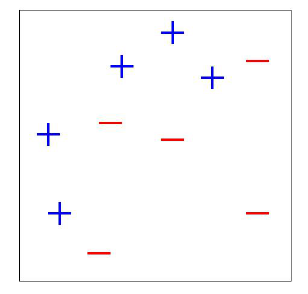
\includegraphics[width=0.6\textwidth]{esempio_adaboost1.png}%
 \caption{\textit{Disposizione dei dati.}}
 \label{grafico1}
\end{figure}
Inizialmente entrambe le popolazioni hanno lo stesso peso. La ``frontiera'' tra le due popolazioni \`e evidente ma non \`e lineare.
\begin{figure}[!h]
\centering
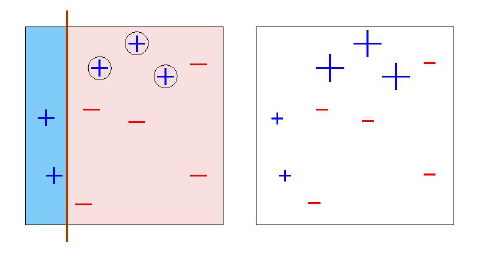
\includegraphics[width=0.8\textwidth]{esempio_adaboost2.png}%
 \caption{\textit{Esito del primo classificatore e conseguente aggiornamento dei pesi.}}
 \label{grafico2}
\end{figure}
\newpage
Individuato il ``primo'' classificatore, possiamo notare come classifica correttamente la classe ``-'', ma commette 3 errori, tali osservazioni verranno
pesate maggiormente al passo successivo. Dalle formule per il calcolo dei coefficienti, 
otteniamo \begin{math}\alpha_1=0.42\end{math}.


\begin{figure}[!h]
\centering
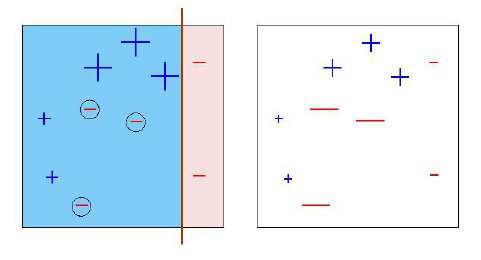
\includegraphics[width=0.8\textwidth]{esempio_adaboost3.png}%
 \caption{\textit{Esito del secondo classificatore e conseguente aggiornamento dei pesi.}}
 \label{grafico3}
\end{figure}

I risultati del secondo classificatore sono analoghi a quelli del primo, \`e di grande importanza, per\`o, notare come variano i pesi delle osservazioni.
Il valore del coefficiente di tale classificatore \`e \begin{math}\alpha_2=0.66\end{math}.
\begin{figure}[!h]
\centering
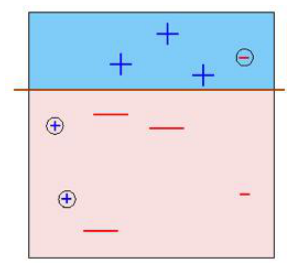
\includegraphics[width=0.6\textwidth]{esempio_adaboost4.png}%
 \caption{\textit{Esito del terzo classificatore.}}
 \label{grafico4}
\end{figure}
\newpage
Introduciamo il terzo classificatore. Questo commette 3 errori, ma i loro pesi sono nettamente inferiori rispetto agli altri,
perch\`e tali osservazioni avevano gi\`a ottenuto un esito corretto dai precedenti classificatori, otteniamo cos\`i un valore per
il coefficiente \begin{math}\alpha_3=0.91\end{math}. Osserviamo i risultati cos\`i ottenuti:


\begin{figure}[!h]
\centering
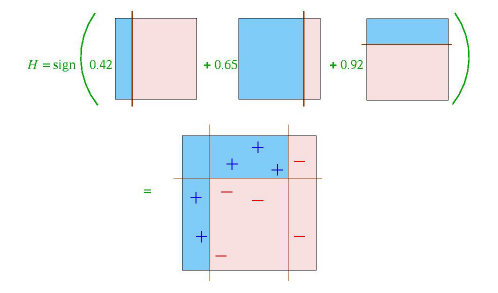
\includegraphics[width=0.9\textwidth]{esempio_adaboost5.png}%
 \caption{\textit{Esito del classificatore finale.}}
 \label{grafico5}
\end{figure}






\chapter{Adaboost Multiclasse}
\ \
\newline
L'algoritmo AdaBoost si pu\`o considerare una grande innovazione per risolvere problemi di Data Mining.
Questo filtro viene applicato per casi dicotomici, ovvero dove le possibili uscite (i possibili risultati)
possono essere due (es. vero/falso, s\`i/no, 1/0, ecc.). In questo capitolo si analizzeranno le estensioni
che permettono di affrontare il caso multivariato ideate dagli stessi creatori del precedente filtro. Il primo chiamato
Adaboost.M1, \`e il ponte necessario per arrivare all'algoritmo che \`e stato fondamentale per le ricerche svolte
nel tirocinio, ovvero Adaboost.M2. Esso infatti parte dalle considerazioni del suo antecedente per migliorarne
la struttura matematica e la performance. In questo capitolo non viene preso ancora 
in considerazione il concetto di multi-label, 
infatti entrambi gli algoritmi hanno, implicitamente, ancora un approccio single-label.
\section{Adaboost.M1}
\ \
\newline
\`E la versione pi\`u semplice tra gli adaboost multiclasse. L'algoritmo prende come input un training set di
\begin{it}m\end{it} esempi \begin{math} D = ((x_1,y_1), . . . , (x_m,y_m)) \end{math} dove \begin{math}x_i\end{math} 
\`e una istanza disegnata da qualche spazio X e rappresentata in qualche maniera (generalmente un vettore di valori attributi),
 e \begin{math}y_i \in Y \end{math} \`e la classe etichetta associata con \begin{math}x_i\end{math}. Si assuma che
il set di possibili etichette Y sia di cardinalit\`a \begin{it}k\end{it}, 
dove \begin{it}k\end{it} \`e sempre un numero intero positivo.\\
\newline
Come nel caso dicotomico, l'adaboost ha la possibilit\`a di interagire con un altro algoritmo non specificato
(chiamato WeakLearn), il quale verr\`a chiamato ripetutamente 
per una serie di iterazioni. Al passo \begin{it}t\end{it}
il booster provvede il WeakLearn con una distribuzione \begin{math}D_t\end{math} sul training set \begin{it}D\end{it}.
 In risposta, il WeakLearn calcola un classificatore o una ipotesi
 \begin{math}h_t : X \times Y \to \left[0,1\right]\end{math} che dovrebbe classificare correttamente
una frazione di training set che ha grande probabilit\`a in relazione 
alla distribuzione \begin{math}D_t\end{math}. Lo scopo del
weak learner \`e quello di trovare un'ipotesi \begin{math}h_t\end{math} che minimizzi l'errore 
\begin{math} \varepsilon_t=Pr{_i\sim D_t} [h_t(x_i\ne y_i)] \end{math}. Questo errore
viene misurato rispetto alla distribuzione \begin{math}D_t\end{math} che \`e stata fornita dal weak learner stesso.
Il processo continua per T volte e, per ultimo, 
il booster combina le ipotesi \begin{math}h_1, ... , h_T\end{math}
in una singola ipotesi finale \begin{math}h_{fin}\end{math}.\\
\newline
Non sono ancora stati specificati il metodo attraverso il quale \begin{math}D_t\end{math} \`e calcolata 
ad ogni iterazione e come \begin{math}h_{fin}\end{math} viene calcolata.
Esistono differenti modi di agire, Adaboost.M1 si comporta come segue:




\begin{itemize}
\item Per una sequenza di \begin{it}m\end{it} esempi di training 
\begin{math}(x_1,y_1), ... (x_m,y_m)\end{math}\\
con etichette \begin{math}y_i\in Y = \left\{1, ..., k\right\}\end{math}
\item Si inizializza il vettore dei pesi: \begin{math} D_1(i)=1/m \end{math}
\item Il processo viene effettuato per T iterazioni
\item Sia \begin{math} \mathcal{L} \end{math} weak learner iniziale
\end{itemize}

\begin{enumerate}
\item Viene chiamato il weak learner fornendolo della distribuzione \begin{math} D_t\end{math}
\item In risposta, il weak learner 
genere un'ipotesi \begin{math} h_t=\mathcal{L}(D,D_t)\end{math} 
\item   \begin{math}\varepsilon = \sum_{i:h_t(x_i)\ne y_i}D_t(i)\end{math} si misura l'errore 
di \begin{math} h_t\end{math}\\
Se \begin{math}\varepsilon>\end{math}1/2, allora T=t-1 e il programma abortisce
                          
\item \begin{math} \alpha_t=\frac{\varepsilon_t}{1-\varepsilon_t}  \end{math} 
determina il peso di \begin{math} h_t\end{math}

\item \begin{math} D_{t+1}(i)=\frac{D_t(i)}{Z_t}\times \begin{cases} \alpha_t &  se  h_t(x_i)=y_i \\ 1 & altrimenti \end{cases}\end{math} \\
\newline
Aggiorna la distribuzione, dove \begin{math}Z_t \end{math} \`e un fattore di normalizzazione (scelto in 
modo tale che \begin{math}D_{t+1} \end{math}
sia una distribuzione).


\end{enumerate}
L'output sar\`a:
\begin{center}
\begin{math} h_{fin}(x)= \underset{y\in Y}{\operatorname{argmax}}\sum_{t:h_t(x)=y} log\frac{1}{\alpha_t} \end{math}
\end{center}








La distribuzione iniziale \begin{math}D_1\end{math} \`e scelta uniforme su \begin{it}D\end{it}, 
quindi \begin{math}D_1\end{math}(i)=1/\begin{it}m\end{it} per tutte le \begin{it}i = 1, ..., m\end{it}.
Per calcolare la distribuzione \begin{math}D_{t+1}\end{math} da \begin{math}D_t\end{math} e l'ultima 
ipotesi weak \begin{math}h_t\end{math}, si moltiplica il peso dell'esempio \begin{it}i\end{it} per 
\begin{math}\alpha_t \in \left[0,1\right)\end{math} se \begin{math}h_t\end{math} classifica \begin{math}x_i\end{math} correttamente, 
altrimenti il peso rimane invariato. I pesi sono poi rinormalizzati dividendo per la costante di normalizzazione
 \begin{math}Z_t\end{math}. 
Con efficacia, esempi ``facili'' che sono stati classificati correttamente prendono 
dalle precedenti ipotesi weak
un peso minore, mentre esempi ``difficili''  che tendono ad essere spesso classificati in 
maniera errata prendono 
un peso maggiore. Perci\`o, adaboost focalizza un peso maggiore sugli esempi che sembrano pi\`u difficili 
per il WeakLearn. \\
\newline
Il valore \begin{math}\alpha_t\end{math} \`e calcolato come funzione dell'errore 
\begin{math}\varepsilon\end{math} secondo il punto (c).  
L'ipotesi finale \begin{math}h_{fin}\end{math} \`e un voto pesato delle ipotesi weak. 
Per una istanza data \begin{it}x\end{it}, \begin{math}h_{fin}\end{math} emette l'etichetta \begin{it}y\end{it} 
che massimizza la somma dei pesi delle ipotesi weak predicendo quella specifica etichetta.
 Il peso delle ipotesi \begin{math}h_t\end{math} \`e definito come \begin{math}\log(\frac{1}{\alpha_t})\end{math},
 ovvero viene dato peso pi\`u grande alle ipotesi con errore pi\`u basso. \\
\newline
Il Teorema 1 dimostra l'importanza teorica di questo algoritmo. 
Esso mostra che se le ipotesi weak in modo compatibile hanno errore solo leggermente migliore di 1/2, 
allora l'errore di training dell'ipotesi finale \begin{math}h_{fin}\end{math} 
si abbassa a zero in maniera esponenziale 
(per il caso di classificazione binaria, questo significa che le ipotesi weak debbano 
essere solo lievemente migliori della casualit\`a).\\
\newline
\textbf{Teorema 1.} Si supponga che l'algoritmo weak, ovvero WeakLearn, quando chiamato dall'Adaboost.M1, 
generi ipotesi con errori \begin{math}\varepsilon_1, ... ,\varepsilon_T\end{math}, dove \begin{math}\varepsilon\end{math} 
\`e definito come illustrato precedentemente. Si assuma ogni \begin{math}\varepsilon <\end{math}1/2 e si ponga 
\begin{math}\gamma_t = 1/2-\varepsilon_t\end{math}. Allora 
l'ipotesi finale \begin{math}h_{fin}\end{math} \`e maggiorata come segue.
\begin{center}
\begin{math}\frac{|\left\{i : h_{fin}(x_i)\ne y_i\right\}|}{m} \le \prod_{t=1}^T\sqrt{1-4\gamma_t^2}
\le exp\left(-2\sum_{t=1}^T\gamma_t^2\right)\end{math}.
\end{center}


Il Teorema 1. implica che l'errore di training\footnote{L'errore di training o errore empirico 
\`e basato sui dati di training, ovvero \`e quello che si commette durante la fase di apprendimento.} 
dell'ipotesi finale generato da M1 \`e piccolo.
Questo per\`o non implica necessariamente che l'errore di test\footnote{L'errore di test \`e l'errore di 
generalizzazione che si stima sui nuovi dati.} 
sia altrettanto piccolo. In pratica l'errore di test tende ad essere 
migliore rispetto a quanto suggerisce la teoria, indicando un chiaro difetto in questa visione teorica.\\
\newline
Il principale svantaggio dell'Adaboost.M1 \`e quello di essere incapace di trattare le weak ipotesi 
con errore superiore a 1/2. L'errore previsto dall'ipotesi che genera casualmente l'etichetta \`e 
1-1/\begin{it}k\end{it}. Quindi, per \begin{it}k\end{it}\begin{math}=\end{math}2, le ipotesi weak hanno bisogno di essere leggermente migliori 
della scelta casuale, ma quando \begin{it}k\end{it}\begin{math}>\end{math}2 (ovvero tutti i casi multidimensionali, per cui
l'M1 \`e stato creato), la richiesta che l'errore sia meno di 1/2 \`e abbastanza forte e spesso pu\`o
 essere difficile da conoscere.
\newpage
\vspace{1.5cm}





\section{Adaboost.M2}
\ \
\newline
Questa versione tenta di superare la difficolt\`a 
trovata nella versione M1 
``aumentando la comunicazione'' tra l'algoritmo di boosting e il weak learner.
Per prima cosa, viene permesso al weak learner di generare pi\`u ipotesi dove, piuttosto che identificare una singola etichetta 
in Y, sceglie un set di ``plausibili'' etichette. Questo pu\`o essere spesso pi\`u facile che sceglierne solo una.
Per esempio, nello scenario OCR, pu\`o esser difficile dire se una particolare immagine \`e un ``7'' o un ``9'', ma \`e
facile eliminare tutte le altre possibilit\`a. In questo caso, piuttosto che decidere tra 7 e 9, il set delle ipotesi pu\`o
essere (7,9), indicando entrambe le etichette plausibili.\\
\newline
 Si permette inoltre al weak learner di dare un grado di plausibilt\`a, cos\`i ogni ipotesi weak dar\`a
un vettore \begin{math} \left [ 0,1 \right ]^k \end{math}, dove le componenti con valori vicini a 0 o a 1 corrispondono
a quelle etichette considerate rispettativamente implausibili o plausibili. Questo vettore non \`e costituito
da probabilit\`a, la somma quindi non necessita di eguagliare a 1.\\
\newline
Mentre l'algoritmo weak acquista maggior potenza espressiva, si mette un requisito sulle performance delle ipotesi
weak pi\`u complesso. Si introduce quindi il concetto di pseudo-loss, che \`e una misura di errore pi\`u
sofisticata. Essa, a differenza degli errori che sono calcolati 
rispetto alle distribuzioni sugli esempi di training,
viene calcolata rispetto alla distruzione sull'insieme di tutte le coppie di esempi e etichette sbagliate.\\
\newline
Vedremo che Adaboost.M2 compie il boosting se 
ogni ipotesi weak ha la pseudo-loss leggermente migliore del calcolo randomizzato. \\
\newline
Per formalit\`a si introduca questo concetto, una \begin{it}mislabel\end{it}  \`e una coppia (\begin{it}i,y\end{it}) dove \begin{it}i\end{it}
 \`e l'indice dell'esempio di training e \begin{it}y\end{it} \`e un'etichetta sbagliata associata 
all'esempio \begin{it}i\end{it}. Sia \begin{it}B\end{it} l'insieme di tutte le \begin{it}mislabel\end{it} 
\begin{math}B=\left\{(i,y) : i \in \left\{1, ..., m \right\}, y \ne y_i \right\}\end{math}. 
Una distribuzione mislabel \`e una distribuzione definita su \begin{it}B\end{it}.\\
\newline

Il procedimento del ciclo Adaboost.M2 \`e il seguente:\\
\newline
\begin{itemize}
\item Per una sequenza di \begin{it}m\end{it} esempi \begin{math}(x_1,y_1), ... (x_m,y_m)\end{math}\\
con etichette \begin{math}y_i\in Y = \left\{1, ..., k\right\}\end{math}
\item Si inizializza il vettore dei pesi: \begin{math} D_1(i)=1/|B| per (i,y) \in B \end{math}
\item Il processo \`e svolto per T volte specificando il numero di iterazioni
\item Sia \begin{math} \mathcal{L} \end{math} weak learner iniziale
\item \begin{math} B=\left\{(i,y) : i \in \left\{1..m\right\},y\ne y_i\right\} \end{math}

\end{itemize}
Per t =1, 2, ..., T:
\begin{enumerate}

\item Viene chiamato il weak learner, fornendolo di una distribuzione
    \begin{math} D_t\end{math} 
\item In risposta, il weak learner genera un'ipotesi  \begin{math}h_t : X \times Y \to \left[0,1\right]\end{math}
\item Viene calcolata la pseudo-loss di \begin{math}h_t\end{math}:
\begin{center}
\begin{math}\varepsilon = \frac{1}{2} \sum_{(i,y)\in B}D_t(i,y)(1-h_t(x_i,y_i)+h_t(x_i,y))\end{math}.
\end{center}                      
\item \begin{math} \alpha_t=\frac{\varepsilon_t}{1-\varepsilon_t}  \end{math} 
determina il peso di \begin{math} h_t\end{math}

\item Si aggiorna \begin{math}D_t\end{math}:
\begin{center}
 \begin{math}
  D_{t+1}(i,y)=\frac{D_t(i,y)}{Z_t}\alpha_t^{(1/2)(h_t(x_i,y_i)-h_t(x_i,y))}
 \end{math}

\end{center}
                             
dove \begin{math}Z_t \end{math} \`e un fattore di normalizzazione che rende \begin{math}D_{t+1} \end{math} 
una distribuzione.


\end{enumerate}
L'output sar\`a:
\begin{center}
\begin{math} h_{fin}(x)= \underset{y\in Y}{\operatorname{argmax}}\sum_{t=1}^T log\frac{1}{\alpha_t}h_t(x,y) \end{math}
\end{center}



Per ogni passo \begin{it}t\end{it} di boosting, Adaboost.M2 fornisce il weak learner con la distribuzione 
mislabel \begin{math}D_t\end{math}. In risposta, il weak learner calcola un'ipotesi \begin{math}h_t\end{math} della 
forma \begin{math}h_t : X \times Y \to \left[0,1\right]\end{math}. Non ci sono restrizioni su
 \begin{math}\sum_y h_t(x,y)\end{math}. In particolare, il vettore predizione non deve essere 
una distribuzione di probabilit\`a. \\
\newline
Intuitivamente, si interpreta ogni mislabel (\begin{it}i,y\end{it}) come rappresentazione di una domanda binaria
 del tipo: ``Predici che l'etichetta associata all'esempio \begin{math}x_i\end{math} sia \begin{math}y_i\end{math}
 (ovvero l'etichetta corretta) o \begin{math}y\end{math} (una tra le etichette sbagliate)?''. 
Con questa interpretazione, il peso \begin{math}D_t(i,y)\end{math} assegnato a questa mislabel rappresenta 
l'importanza di distinguere l'etichetta sbagliata \begin{math}y\end{math} dall'esempio \begin{math}x_i\end{math}.\\
\newline
Un'ipotesi weak \begin{math}h_t\end{math} viene poi interpretata nella maniera seguente. Se \begin{math}h_t(x_i,y_i)=1\end{math}
 e \begin{math}h_t(x_i,y)=0\end{math} allora \begin{math}h_t(i,y)\end{math} ha (correttamente) predetto che l'etichetta 
di \begin{math}x_i\end{math} sia \begin{math}y_i\end{math} e non \begin{math}y\end{math} (\begin{math}h_t\end{math} 
ritiene \begin{math}y_i\end{math} essere ``plausibile'' e \begin{math}y\end{math} ``non plausibile''. 
In maniera analoga, \begin{math}h_t(x_i,y_i)=0\end{math} e \begin{math}h_t(x_i,y)=1\end{math} allora
 \begin{math}h_t(i,y)\end{math} ha fatto la predizione sbagliata. 
Se \begin{math}h_t(x_i,y_i) = h_t(x_i,y)\end{math} allora la predizione di \begin{math}h_t\end{math} \`e 
fatta arbitrariamente.\\
\newline
Questa interpretazione porta a definire la psudo-loss dell'ipotesi \begin{math}h_t\end{math} rispetto alla 
distribuzione mislabel \begin{math}D_t\end{math} come:
\begin{center}
\begin{math}\varepsilon = \frac{1}{2} \sum_{(i,y)\in B}D_t(i,y)(1-h_t(x_i,y_i)+h_t(x_i,y))\end{math}.
\end{center}
Pu\`o essere verificato che la pseudo-loss \`e minimizzata quando le etichette corrette \begin{math}y_i\end{math}
 sono assegnate al valore 1 e le etichette scorrette \begin{math}y\ne y_i\end{math} al valore 0.\\
\newline
Lo scopo del weak learner \`e quello di trovare un'ipotesi \begin{math}h_t\end{math} con una pseudo-loss piccola. 
Perci\`o, gli algoritmi ``standard'' \`e possibile che abbiano bisogno di qualche modifica per essere usati 
in questa maniera. Dopo avere ricevuto \begin{math}h_t\end{math}, 
la distribuzione mislabel \`e aggiornata usando una regola simile a quella utilizzata nell'Adaboost.M1. 
L'ipotesi finale \begin{math}h_{fin}\end{math} restituisce come output, per un'istanza data \begin{it}x\end{it}, 
l'etichetta \begin{it}y\end{it} che massimizza la media pesata delle ipotesi weak \begin{math}h_t(x,y)\end{math}.\\
\newline
Il seguente teorema pone un limite superiore all'errore di training dell'ipotesi finale. Si noti che questo teorema 
necessita solo che le ipotesi weak abbiano la pseudo-loss minore di 1/2, senza considerare il numero delle classi.
Nonostante le ipotesi weak siano state stimate rispetto alla pseudo-loss, si \`e certamente stimata l'ipotesi 
finale utilizzando l'errore di misura ordinario.\\
\newline
\textbf{Teorema 2.} Si supponga un classificatore debole WeakLearn, che quando viene chiamato dall'Adaboost.M2, 
generi ipotesi con la pseudo-loss \begin{math}\varepsilon_1, ... ,\varepsilon_T\end{math}, dove \begin{math}\varepsilon\end{math}
\`e definita come nello schema precedente. Sia \begin{math}\gamma_t = \frac{1}{2}-\varepsilon_t\end{math}.
 Allora il margine superiore dell'ipotesi finale \begin{math}h_{fin}\end{math}:
\begin{center}
\begin{math}\frac{|\left\{i : h_{fin}(x_i)\ne y_i\right\}|}{m} \le (k-1)\prod_{t=1}^T\sqrt{1-4\gamma_t^2}
\le (k-1)exp\left(-2\sum_{t=1}^T\gamma_t^2\right)\end{math}. 
\end{center}


dove k \`e il numero di classi.\\








\chapter{Generalizzazioni per affrontare il problema multi-label}
\ \
\newline
In questo capitolo verranno analizzati due modelli che tengono conto del concetto multi-label. Il primo, chiamato 
SAMME, aggiunge una costante additiva nel calcolo della funzione dell'errore per la 
creazione di un nuovo modello; il secondo, chiamato Adaboost.MH, parte dalle considerazioni del filtro M2 
per sviluppare un nuovo concetto di errore. 
\section{Forward Stagewise Additive Modeling}
\ \
\newline
Prima di arrivare ad enunciare gli algoritmi che verranno trattati in questo capitolo, si introduce il concetto 
di Forward Stagewise Additive Modeling, che in italiano potrebbe essere tradotto come modello addittivo svolto per 
passaggi in avanti, dove un modello addittivo generale, si ottimizza attraverso la forward stagewise.\\
\newline
Molti modelli di classificazione e regressione possono essere scritti come combinazione lineare di modelli 
pi\`u semplici:
\begin{center}
 \begin{math}
  f(x)=\sum_{m=1}^M \beta_m b_m (x,\gamma_m)
 \end{math}
\end{center}
Dove:
\begin{itemize}
 \item x \`e un dato di imput
 \item \begin{math}
        \left\{ \beta_m,\gamma_m\right\}
       \end{math} sono parametri del modello
 \item \begin{math}
         b_m(x,\gamma_m)
       \end{math} sono altre funzioni arbitrarie di x

\end{itemize}
Generalmente,\begin{math} \left\{ \beta_m,\gamma_m\right\}\end{math} sono stimate per minimizzare alcune
loss function L, che misurano l'errore di predizioni sui dati di training. Spesso questo procedimento 
risulta essere piuttosto complicato, se per\`o si ottimizza la funzione su una funzione base del tipo:
\begin{center}
 \begin{math}
  min \sum_{i=1}^N L(y_i,\beta b_m(x_i,\gamma)
 \end{math}
\end{center}
pu\`o essere risolto il problema. In altri termini l'idea \`e, aggiungere sequenzialmente nuove funzioni base 
per l'espansione della funzione \begin{math}f(x)\end{math} senza cambiare i parametri che sono stati aggiunti.\\
\newline
L'adaboost fitta un modello addittivo, attraverso il modello forward stagewise, dove:
\begin{itemize}
 \item La funzione base \begin{math}b_m\end{math} \`e un classificatore binario
 \item La funzione oggetto \`e la loss esponenziale
\begin{center}
\begin{math} L(y,f) = e^{-yf(x)} \end{math}
\end{center}
\end{itemize}


\section{SAMME}
\ \
\newline
Prima di commentare le particolarit\`a di questa variante, si espone un breve schema riguardante 
i passaggi principali dell'algoritmo:\\
\newline

\begin{itemize}
\item Si inizializza il vettore dei pesi: \begin{math} D_1(i)=1/m \end{math}
\item Il processo viene effettuato per T iterazioni
\item Sia \begin{math} \mathcal{L} \end{math} il classificatore weak iniziale
\end{itemize}

\begin{enumerate}
\item Viene chiamato il weak learner \begin{math} \mathcal{L} \end{math}
 \item In risposta, esso genera \begin{math} h_t \end{math} per i dati di 
training usando i pesi
\item \begin{math} \varepsilon_t = \sum_{i=1}^m D_t(i) 
\mathbbm{1}(c_i\ne h_t(x_i))/\sum_{i=1}^m D_t(i)\end{math}   misura l'errore
\item \begin{equation} \label{eq:alg} 
\alpha_t=\frac{1}{2}\ln\frac{1-\varepsilon_t}{\varepsilon_t} + log(K-1) \end{equation} 

\item Si assegna:
\begin{center}
 \begin{math}
  D_t(i) \leftarrow D_t(i) 
 \end{math} exp\begin{math}
                (\alpha_t\mathbbm{1}(c_i\ne h_t(x_i))
               \end{math}, i = 1, ..., m


\end{center}

\item Ri-normalizza \begin{math}
                     D_i(t)
                    \end{math}


\end{enumerate}
L'output sar\`a:
\begin{center}
 \begin{math} C(x)= \underset{k}{\operatorname{argmax}}\sum_{(t=1)}^T \alpha_t  
\mathbbm{1}(h_t(x) = k)\end{math}
\end{center}


SAMME assomiglia molto alle versioni Adaboost, con la principale differenza in (\ref{eq:alg}). 
Adesso in modo tale da avere \begin{math}\alpha_t\end{math} positivo, 
si ha necessit\`a solo che \begin{math}1-\varepsilon_t >\end{math}1/K, o che l'accuratezza di 
ogni classificatore weak sia migliore della classificazione casuale piuttosto che 1/2. 
Come conseguenza, questo algoritmo pone pi\`u peso sulle osservazioni mal classificate in due dimensioni 
rispetto agli adaboost standard, e inoltre esso combina i classificatori weak in maniera leggermente diversa, 
ovvero per \begin{math}\log(K-1)\sum_{t=1}^T \mathbbm{1}(h_t(x) = k)\end{math}.\\
\newline
Nel caso di k=2, ovvero il caso a due classi, la costante addittiva di SAMME diventa un valore pari a 0 
(essendo il logaritmo di 1), 
l'algoritmo si riduce quindi al ``classico'' adaboost. Questo termine extra, come sar\`a spiegato in maniera 
esaustiva nella prossima sezione, non \`e artificiale e crea un nuovo algoritmo 
equivalente a fittare un modello addittivo in forward 
stagewise attraverso la loss function esponenziale. La differenza tra SAMME e Adaboost (quando k=3) 
\`e anche illustrata in Figura 1.\\

\vspace{1.5cm}
\begin{figure}
 \makebox[\textwidth][c] {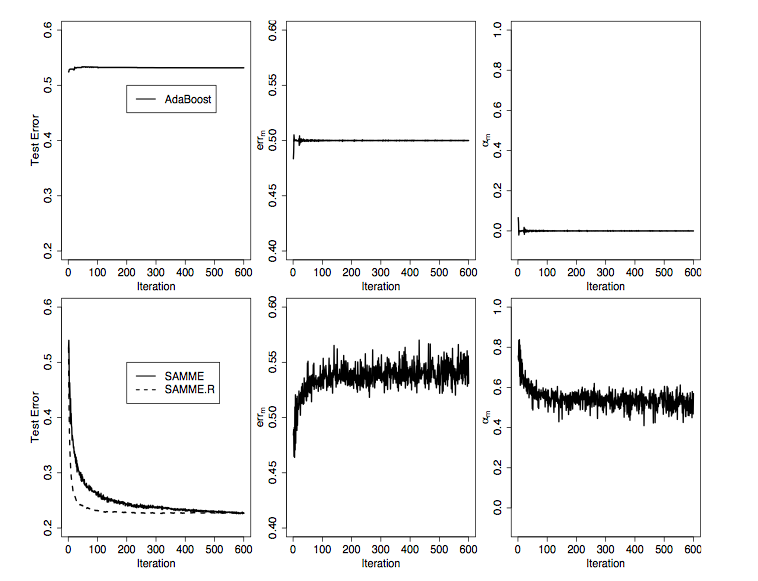
\includegraphics[width=1.0\textwidth]{confronto_samme_m2.png}}%
 \caption{Confronto grafico fra Adaboost (prima riga) 
e SAMME (seconda riga) su una semplice simulazione a tre classi. La taglia di 
training \`e 3000, mentre la taglia di test \`e 10000. Sono stati utilizzati come classificatori weak dieci 
alberi di decisione.}
 \label{fig:key}
\end{figure}

Come \`e gi\`a stato detto, Adaboost si arresta dopo che l'errore supera 1/2. Questo non riguarda SAMME: 
anche se l'errore diventasse maggiore (o uguale) a 1/2, il 
valore \begin{math}\alpha \end{math} sarebbe ancora positivo; 
da ci\`o, gli esempi di training classificati in maniera errata prendono pi\`u peso, 
e l'errore di test si mantiene 
decrescente anche dopo 600 iterazioni. \\
\newline
\subsection{Giustificazione teorica}
Come accennato in precedenza la costante additiva 
\begin{math}\log(K-1)\end{math} in (\ref{eq:alg}) non 
\`e artificale, crea un filtro equivalente a fittare un modello addittivo 
attraverso la forward stagewise. Friedman svilupp\`o una prospettiva statistica sull'originale algoritmo adaboost 
a due classi, che induce a vedere l'adaboost a due classi come un modello addittivo 
forward stagewise attraverso la funzione loss esponenziale:
\begin{center}
\begin{math} L(y,f) = e^{-yf(\textbf{x})} \end{math}
\end{center}
dove \begin{math}y=(\mathbbm{1}(y = 1) - \mathbbm{1}(y = 2))\in \left\{-1,1\right\}\end{math} 
in un ambiente di classificazione a due classi. Non \`e difficile mostrare che l'argmin 
della funzione loss esponenziale \`e la met\`a della trasformazione logit: 
\begin{center}
 \begin{math} f^*(\textbf{x})=\underset{f(\textbf{x})}{\operatorname{argmin}}L(y,f)= 
\frac{1}{2}\end{math}
           \begin{math}\frac{(Prob (y) =1|\textbf{x})}{(Prob (y)=2|\textbf{x})}\end{math}
\end{center}
La regola di classificazione ottimale di Bayes concorda col segno di \begin{math}f^*(x)\end{math}, ovvero
\begin{center}
 \begin{math}
 \underset{y}{\operatorname{argmax}} 
 \end{math} Prob\begin{math}
                 (Y=y | \textbf{X=x}) =
                \end{math} sign\begin{math}
                                (f^*(\textbf{x}))
                               \end{math}



\end{center}

\subsection{Nuova loss function multiclasse}
In un ambiente di classificazione multiclasse, si pu\`o ricodificare l'output \begin{it}y\end{it} 
con un vettore \textbf{y} \begin{it}K\end{it}-dimensionale, 
dove tutte le entrate sono uguali a \begin{math}-\frac{1}{K-1} \end{math}
 eccetto a 1 in posizione \begin{it}k \end{it} se \begin{it}c=k\end{it}, 
cio\`e \begin{math} \textbf{y} =(y_1,...,y_K)^t\end{math} e:
\begin{center}
 \begin{equation}\label{eq:vet_mc}
 y_k=\begin{cases}1 & y=k\\
-\frac{1}{K-1} & y\ne k\end{cases}
\end{equation}
\end{center}
La stessa architettura \`e stata utilizzata in altri ambienti come ad esempio nella versione multiclasse di 
support vector machine (SVM).\\
\newline
La generalizzazione della funzione loss esponenziale al caso multivariato segue naturalmente:
 \begin{center}
 \begin{equation} \label{eq:loss_mc}
L(\textbf{y,f}) =
exp(-\frac{1}{K}(y_1f_1 + ... + y_Kf_K)) = (-\frac{1}{K}\begin{bf}y^tf\end{bf})
\end{equation}
\end{center}
dove \begin{math}f_k\end{math} corrisponde alla classe \begin{it}k\end{it}.\\
\newline
Si noti che c'\`e bisogno di alcuni vincoli su \begin{bf}f\end{bf} affinch\`e (\ref{eq:loss_mc}) 
sia stimabile, d'altra parte, 
aggiungendo qualsiasi costante a tutto \begin{math}f_k\end{math} non cambia la perdita (loss). Viene scelto di usare il 
vincolo di simmetria:
\begin{center}
 \begin{math} f_1 + ... + f_K = 0
\end{math}
\end{center}
In questo modo, quando K=2 la funzione loss esponenziale multinomiale si riduce alla funzione loss esponenziale 
classica biclasse.\\
\newline
In maniera simile al caso a due classi, si \`e interessati a scoprire cosa questa funzione loss esponenziale 
multiclasse stimi. A questo si pu\`o rispondere cercando il suo argmin. 
In particolare, si \`e interessati a:
\begin{center}
 \begin{math} \underset{\begin{bf}f(x)\end{bf}}{\operatorname{argmin}}\end{math} 
E\begin{math}_{\begin{bf}Y|x\end{bf}} \end{math}exp
\begin{math}(-\frac{1}{K}(Y_1f_1 + ... + Y_Kf_K))
\end{math}
\end{center}
\begin{center}
 soggetto al vincolo \begin{math}f_1 + ... + f_K = 0
\end{math}
\end{center}
Segue dai calcoli:
\begin{center}
\begin{math}
exp (-\frac{1}{K}( f_1(\textbf{x}) - \frac{f_2(\textbf{x})}{K-1} - \dots - \frac{f_K(\textbf{x})}{K-1}) Prob ((y)=1|\textbf{x}) + 
\dots  
\end{math}
\end{center}

\begin{center}
 \begin{math}
  + exp (-\frac{1}{K}( \frac{f_1(\textbf{x})}{K-1} - \frac{f_2(\textbf{x})}{K-1} - \dots - f_K(\textbf{x}) 
Prob ((y)=K|\textbf{x}) =
 \end{math}
\end{center}

\begin{center}
 \begin{math}
  exp(-\frac{1}{K}(F_1(\textbf{x}) + \frac{f_1(\textbf{x})}{K-1})) Prob ((y)=K|\textbf{x})
 \end{math}

\end{center}


\begin{center}
 \begin{math}
  + exp(-\frac{1}{K}(f_K(\textbf{x}) + \frac{f_K(\textbf{x})}{K-1})) Prob ((y)=K|\textbf{x})
 \end{math}

\end{center}


Attraverso il metodo dei moltiplicatori di Lagrange questo problema di ottimizzazione vincolata pu\`o 
esser riscritto come:
\begin{center}
 \begin{math}
  exp (-\frac{f_1(\textbf{x})}{K-1} Prob((y)=1|\textbf{x})) + \dots 
+ exp (-\frac{f_K(\textbf{x})}{K-1} Prob((y)=K|\textbf{x})) + 
 \end{math}
\end{center}
\begin{center}
 \begin{math}
-  \lambda (f_1(\textbf{x}) + \dots + f_K(\textbf{x})
 \end{math}

\end{center}
dove \begin{math}
      \lambda 
     \end{math}  \`e il moltiplicatore di Lagrange. Calcolando le derivate rispetto a 
\begin{math}
 f_k
\end{math} e \begin{math}
              \lambda
             \end{math}, troviamo:
\begin{center}
 \begin{math}
  -\frac{1}{K-1} exp (-\frac{f_1(\textbf{x})}{K-1} Prob((y)=1|\textbf{x}) -\lambda = 0
 \end{math}

\end{center}
\begin{center}
 \begin{math}
 \vdots
\end{math}
\end{center}

\begin{center}
 \begin{math}
  -\frac{1}{K-1} exp (-\frac{f_K(\textbf{x})}{K-1} Prob((y)=K|\textbf{x}) -\lambda = 0
 \end{math}
\end{center}
\begin{center}
 \begin{math}
  f_1 + ... + f_K = 0
 \end{math}

\end{center}

Risolvendo questo sistema di equazioni, si ottiene:
\begin{center}
 \begin{equation}\label{eq:lagrange}
 f_k^*(\textbf{x}) = (K-1) (log Prob(c=k|\textbf{x}) - \frac{1}{K}\sum_{k'=1}^K log Prob(y=k'|\textbf{x}))
\end{equation}
\end{center}
con k=1,...,K; perci\`o:
\begin{center}
 \begin{math} \underset{k}{\operatorname{argmax}} f_k^*(\textbf{x}) = 
\underset{k}{\operatorname{argmax}}Prob(c=k|\textbf{x})
\end{math}
\end{center}
che \`e la regola di classificazione ottimale di Bayes per l'errore. Questo giustifica l'uso della 
funzione loss esponenziale multiclasse. L'equazione (\ref{eq:lagrange}) trova anche un modo per recuperare 
\begin{math}
 Prob( y = k | \textbf{x})
\end{math} una volta che \begin{math}
                          f^*_k(\textbf{x})
                         \end{math} sono stimate:
\begin{center}
 \begin{math}
  Prob( c = k | \textbf{x}) = \frac{exp(\frac{1}{K-1}f^*_k(\textbf{x}))}{exp(\frac{1}{K-1}f^*_1(\textbf{x}))+ ... + 
exp(\frac{1}{K-1}f^*_k(\textbf{x}))}
 \end{math}
 per k =1, ..., K
\end{center}


\subsection{SAMME e FSAM}
Adesso si mostrer\`a che l'algoritmo SAMME \`e equivalente al modello addittivo per forward stagewise utilizzando 
la loss function esponenziale multiclasse trovata nel paragrafo precedente (\ref{eq:loss_mc}). Inizialmente si lavorer\`a con la loss function 
canonica, successivamente verr\`a applicata quella multiclasse.\\
\newline
Avendo dei dati di training, ci auguriamo di trovare \begin{math}f(\textbf{x}) = 
(f_1(\textbf{x})+ ...+ f_K(\textbf{x}))^t \end{math} tale che:
\begin{center}
 \begin{equation}\label{eq:minimo}
 \underset{f(\textbf{x})}{\operatorname{min}} \sum_{i=i}^mL(\textbf{y}_i,f(\textbf{x}_i))
\end{equation}
\end{center}

 soggetto al vincolo
\begin{center} 
\begin{equation}\label{eq:vincolo}
f_1(\textbf{x}) + ... + f_K(\textbf{x}) = 0
\end{equation}
\end{center}
Si consideri \begin{math}
              f(\textbf{x})
             \end{math} che ha la seguente forma:
\begin{center}
 \begin{math} f(\textbf{x}) = \sum_{t=1}^T\beta_t g_t(\textbf{x})
\end{math}
\end{center}
dove \begin{math}
      \beta_t \in \mathbb{R}
     \end{math} sono coefficienti e \begin{math}
                                    g_t(\textbf{x})
                                   \end{math} sono funzioni base. Ordiniamo a \begin{math}
                                    g_t(\textbf{x})
                                   \end{math} 
di soddisfare il vincolo \begin{math}g_1(\textbf{x}) + ... + g_K(\textbf{x}) = 0
\end{math}.\\
\newline 
Per esempio,la funzione \begin{math}
                                    g_t(\textbf{x})
                                   \end{math} che si considera prende valore in uno dei K possibili vettori 
K-dimensionali; precisamente, dato \begin{math}\textbf{x}\end{math}, 
\begin{math}\textbf{g(x)}\end{math} mappa \begin{math}\textbf{x}\end{math} su \begin{math}
                                                                               \mathcal{Y}
                                                                              \end{math}
\begin{center}
 \begin{math}
  g: \textbf{x} \in \mathbb{R}^p \rightarrow \mathcal{Y}
 \end{math}

\end{center}
dove \begin{math}
      \mathcal{Y}
     \end{math} contiene K vettori K-dimensionali.




Il modello forward stagewise approssima la soluzione delle richieste (\ref{eq:minimo})-
(\ref{eq:vincolo}) sequenzialmente 
aggiungendo nuove funzioni base all'espansione senza adattare i parametri e coefficienti di quelli che erano 
gi\`a stati aggiunti. Specificatamente, l'algoritmo parte con \begin{math}
                                                               f_0(\textbf{x}) = 0
                                                              \end{math} sequenzialmente seleziona nuove 
funzioni base da un dizionario e le aggiunge:
\begin{itemize}
 \item Inizializza \begin{math}f_0(x) = 0 \end{math}
\item Per \begin{math}t = 1 ... T \end{math} iterazioni\\
\newline
Calcola:
\begin{center}
 \begin{math} (\beta_t,g_t(\textbf{x})) = \underset{\beta,g}{\operatorname{min}}
\sum_{i=1}^m L(\textbf{y}_i, f_{t-1}(\textbf{x}_i) + \beta g(\textbf{x}_i))
\end{math}
\end{center}
Assegna:
\begin{center}
 \begin{math} f_t(\textbf{x}) = f_{(t-1)}(\textbf{x}) + \beta_t g_t(\textbf{x})
\end{math}
\end{center}
\end{itemize}
Il passo cruciale di questo studio avviene al calcolo di  \begin{math} (\beta_t,g_t)
\end{math}, infatti, usando la funzione loss esponenziale multivariata:
\begin{center}
 \begin{equation} \label{eq:sol1}
(\beta_t,g_t) = \underset{\beta,g}{\operatorname{argmin}} \sum_{i=i}^m exp(
-\frac{1}{K}\textbf{y}_i^t(f_{t-1}(\textbf{x}_i) + \beta g(\textbf{x}_i))\end{equation}
\end{center}
\begin{center}
 \begin{equation}\label{eq:sol2}
= \underset{\beta,g}{\operatorname{argmin}} \sum_{i=1}^m D_t(i) exp(
 -\frac{1}{K}\beta \textbf{y}_i^tg(\textbf{x}_i))
\end{equation}                                                                      
\end{center}
dove \begin{math}D_t(i) =\end{math} exp \begin{math}-\frac{1}{K}\textbf{x}_i^t(f_{t-1}(\textbf{x}_i)\end{math} sono i pesi non 
normalizzati.\\
\newline
Si noti che ogni funzione \begin{math}
                           g(\textbf{x})
                          \end{math} nei K vettori K-dimensionali ha una corrispondenza con un classificatore 
multiclasse \begin{math}
             h(x)
            \end{math}
 come segue:
\begin{center}
 \begin{equation}\label{eq:cor1}
  h(x) = k, 
 \end{equation}
se \begin{math} g_k(\textbf{x})=1\end{math}
                                 
\end{center}
e vice versa.

Quindi, risolvere \begin{math}g_t(\textbf{x})\end{math} \`e equivalente a trovare il classificatore multi-classe 
\begin{math}h_t(x)\end{math} che pu\`o generare \begin{math}g_t(\textbf{x})\end{math}. Di seguito si proceder\`a 
quindi con lo svolgimento della soluzione:
\begin{center}
\begin{equation}\label{eq:T_m}
 h_t (\textbf{x})= argmin  \sum_{i=1}^m D_t(i) \mathbbm{1}(y_i\ne h(\textbf{x}_i))
\end{equation}                                                                      
\end{center}
\begin{center}
\begin{equation}\label{eq:beta_m}
\beta_t = \frac{(K-1)^2}{K} ( log \frac{1-\varepsilon_t}{\varepsilon_t} + log(K-1)
\end{equation}                                                                      
\end{center}
Dove \begin{math}\varepsilon_t\end{math} \`e definito come :
\begin{center}
\begin{math}
 \varepsilon_t = \sum_{i=1}^m D_t(i) \mathbbm{1}(c_i\ne h(\textbf{x}_i))/\sum_{i=1}^m D_t(i)
\end{math}                                                                      
\end{center}
Adesso, per ogni valore fissato \begin{math}
                                 \beta >0
                                \end{math}, utilizzando la definizione (\ref{eq:cor1})
 
si pu\`o esprimere il criterio in (\ref{eq:sol2}) come:

\begin{center}
\begin{math}
 \sum_{y_i=h(x_i)}D_t(i)\end{math}exp
\begin{math}(-\frac{\beta}{K-1} - \sum_{y_i\ne h(x_i)}D_t(i)\end{math}exp
\begin{math}(\frac{\beta}{(K-1)^2})=
\end{math}                                                                      
\end{center}
\begin{center}
\begin{equation}\label{eq:sol3}
 exp(-\frac{\beta}{K-1}\sum_i D_t(i) + (exp
(\frac{\beta}{(K-1)^2}) - exp
(\frac{\beta}{K-1}))\sum_i^m D_t(i)
\end{equation}                                                                      
\end{center}
Solo l'ultima somma dipende dal classificatore \begin{math}h(\textbf{x})\end{math}, 
noi prendiamo quella che contiene la (\ref{eq:T_m}). 
A questo punto, inserendo (\ref{eq:T_m}) in (\ref{eq:sol2}) e risolvendo per \begin{math}
                                 \beta
                                \end{math}, si ottiene (\ref{eq:beta_m}).\\
\newline
Il modello viene poi aggiornato:
\begin{center}
\begin{math}
 f_t(\textbf{x}) = f_{t-1}(\textbf{x}) + \beta_t g_t(\textbf{x})
\end{math}                                                                      
\end{center}
e i pesi per la prossima iterazione saranno:
\begin{center}
\begin{math}
 D_t(i) \leftarrow D_t(i)\end{math} exp
 \begin{math}(-\frac{1}{K}\beta_t y_i^tg_t(\textbf{x}_i)) \end{math}                                                                   
\end{center}
Questo equivale a:
\begin{center}
\begin{equation}\label{eq:finale}
 D_t(i) exp(-\frac{(K-1)^2}{K^2} \alpha_t y_i^t g_t(\textbf{x}_i) )
= \begin{cases}D_t(i) exp(-\frac{(K-1)^2}{K} \alpha_t) & y_i=h(x_i)\\
  D_t(i) exp(\frac{1}{K}\alpha_t) & y_i\ne h(x_i) 
  \end{cases}
\end{equation}                                                                      
\end{center}
Dove \begin{math}\alpha_t \end{math} \`e definita in (\ref{eq:alg}) col termine extra log(K-1), e il nuovo peso 
\`e equivalente al peso dell'algoritmo SAMME aggiornato dopo la normalizzazione.




\section{Adaboost.MH}
Adaboost.MH \`e una generalizzazione del filtro M2. Potendo la singola osservazione x appartenere a diverse 
etichette (concetto multi-label), 
si introduce un nuovo algoritmo che, con diversi concetti di funzione loss, affronta la possibilit\`a 
di cambiamento delle label. Si 
noti, come si mostrer\`a in questo paragrafo, che nel caso ogni osservazione appartenga a una sola classe, questo 
filtro si riduce ad Adaboost.M2.\\
\newline
Sia \begin{math}
     Y 
    \end{math} un set finito di etichette, e sia \begin{math}
                                                           k = |Y|
                                                          \end{math}. In un ambiente di classificazione 
tradizionale, ogni esempio \begin{math}
     x \in X 
    \end{math} alla singola classe \begin{math}
     y \in Y 
    \end{math}, quindi gli esempi etichettati sono coppie \begin{math}
                                                           (x,y)
                                                          \end{math}. Lo scopo poi, generalmente, 
\`e di trovare un'ipotesi \begin{math}
                         H : X \rightarrow Y
                        \end{math} che minimizza la probabilit\`a che \begin{math}
                                                                       y \ne H(x)
                                                                      \end{math} su un nuovo 
esempio osservato \begin{math}  (x,y) \end{math}. \\
\newline
Nel caso multi-label, ogni istanza \begin{math}
     x \in X 
    \end{math} pu\`o appartenere a diverse classi in \begin{math}
                                                      Y
                                                     \end{math}. Quindi, un esempio etichettato \`e una coppia 
\begin{math}(x,\mathcal{Y})\end{math} dove \begin{math}
                                  \mathcal{Y} \subseteq Y
                                 \end{math} nel set di etichette assegnate a x. Il caso single-label \`e 
chiaramente un caso speciale quando \begin{math} |Y| = 1   \end{math} per tutte le osservazioni.\\
Non \`e chiaro in questo ambiente precisamente come formalizzare lo scopo dell'algoritmo di apprendimento, e, in 
generale, la ``giusta'' formalizzazione pu\`o dipendere dal problema. Una possibilit\`a \`e di cercare un'ipotesi 
che prova a predire solo una delle etichette assegnate a un esempio. In altre parole, lo scopo \`e di trovare 
\begin{math} H : X \rightarrow Y\end{math} che minimizza la probabilit\`a che 
\begin{math}
 H(x) \notin \mathcal{Y}
\end{math} su una nuova osservazione \begin{math}
                                      (x,\mathcal{Y})
                                     \end{math}. Chiamiamo questa misura ``un errore'' delle ipotesi 
\begin{it}H\end{it} siccome misura la probabilit\`a di non ottenere anche una tra le etichette corrette. 
Si denota ``un errore'' di un'ipotesi \begin{it}h\end{it} rispetto alla distribuzione \begin{it}D\end{it} 
sulle osservazioni \begin{math}(x,\mathcal{Y})\end{math} in questo modo:
\begin{center}one-err
 \begin{math}
  _D(H) = Pr_{(x,Y) \texttildelow D}\left[H(x) \notin \mathcal{Y}\right]
 \end{math}

\end{center}
Si noti che, per un problema di classificazione single-label, ``un errore'' \`e il corrispondente dell'errore 
ordinario. Nel paragrafo seguente, si introdurr\`a una nuova misura di perdita (loss) che pu\`o essere utilizzata 
in questo ambiente multiclasse, chiamata Hamming loss (o ranking loss). Si analizzeranno inoltre le modifiche 
appropriate all'Adaboost per via di questo nuovo concetto di perdita (loss).

\subsection{Utilizzo della Hamming loss per i problemi multi-classe}
Si supponga adesso che lo scopo sia di predire tutte e solo le etichette corrette. Ovvero, l'algoritmo 
di apprendimento genera un'ipotesi che predice sets di etichette, e la loss dipende su come queste predizioni 
differiscono da una che \`e stata osservata. Perci\`o, 
\begin{math} H : X \rightarrow 2^Y\end{math} e, rispetto alla distribuzione \begin{it} D\end{it} 
la loss \`e:
\begin{center}
 \begin{math}
 \frac{1}{k} E_{(x,Y) \texttildelow  D} \left[|h(x) \mathcal{4} \mathcal{Y} | \right]
 \end{math}
\end{center}
dove \begin{math}
      \mathcal{4}
     \end{math} denota la differenza simmetrica (il valore 1/k \`e utilizzato solo per assicurarsi che 
il valore stia in \begin{math}
                   \left[0,1\right]
                  \end{math}). Chiamiamo questa misura \begin{it}
                                                        Hamming loss
                                                       \end{it} di H, e la denotiamo come
\begin{math}
 hloss_D(H)
\end{math}. Per minimizzare la Hamming loss, si pu\`o, in maniera naturale, decomporre il problema in 
\begin{it}k\end{it} problemi di classificazione binaria ortogonali. Si pensa a 
\begin{math}\mathcal{Y}\end{math} come \begin{it}k\end{it} 
etichette binarie (dipendendo da che un'etichetta \begin{it}y\end{it} sia o 
non sia inclusa in \begin{math}\mathcal{Y}\end{math}). 
Similmente, \begin{it}h(x)\end{it} pu\`o essere vista come \begin{it}k\end{it} predizioni binarie. 
La Hamming loss poi pu\`o essere considerata come una media dell'errore di \begin{it}h\end{it} su questi 
\begin{it}k\end{it} problemi binari. \\
Per  \begin{math} \mathcal{Y} \subseteq Y \end{math}, si definisce \begin{math}
                                                                    \mathcal{Y}\left[l\right]
                                                                   \end{math} per \begin{math}
                                                                                   l \in Y
                                                                                  \end{math} essere:
\begin{center}
 \begin{math}
   \mathcal{Y}\left[l\right] = \begin{cases}1 & l \in \mathcal{Y}\\
-1 & l\notin \mathcal{Y}\end{cases}
 \end{math}

\end{center}
Per semplificare la notazione, si identifica anche qualsiasi funzione 
\begin{math} H : X \rightarrow 2^Y\end{math} con una corrispondente funzione a due 
argomenti \begin{math}
           H : X \times Y \rightarrow \left\{-1,1\right\}
          \end{math} definita da \begin{math}
                                  H(x,l) = H(x)\left[l\right]
                                 \end{math}\\
\newline
Con la riduzione alla classificazione binaria in mente, \`e piuttosto inequivocabile vedere come utilizzare 
il boosting per minimizzare la Hamming loss. L'idea principale della riduzione \`e semplicemente ripetere ogni 
esempio di training \begin{math}
                     (x_i,Y_i)
                    \end{math} per \begin{it}k\end{it} esempi 
\begin{math}
 ((x_i,l),Y_i\left[l\right])
\end{math} per \begin{math}
                l \in \mathcal{Y}
               \end{math}. Il risultato \`e un algoritmo di boosting chiamato proprio Adaboost.MH che mantiene 
una distribuzione sugli esempi \begin{it}i\end{it} e etichette \begin{it}l\end{it}.\\
Come per ogni classificatore, si riporta un breve schema con i passaggi essenziali dell'algoritmo.
\begin{itemize}
 \item Dati: \begin{math}
              (x_1,Y_1), ..., (x_m,Y_m)
             \end{math} dove \begin{math}
                              x_i \in X, \mathcal{Y}_i \subseteq Y
                             \end{math}
 \item Si inizializza \begin{math}
                       D_1(i,l) = 1/(mk)
                      \end{math}
 \item Per t = 1, ..., T
\end{itemize}

\begin{enumerate}
 \item Viene chiamato il weak learner utilizzando la distribuzione \begin{math}
                                                             D_t
                                                            \end{math}
 \item Il weak learner, in risposta, genera un'ipotesi \begin{math}
                               h_t : X \times Y \rightarrow \mathbb{R}
                              \end{math}
 \item Viene calcolato \begin{math}
                \alpha_t \in \mathbb{R}
               \end{math}
 \item Viene aggiornata:

\end{enumerate}
\begin{center}
 \begin{math}
  D_{t+1}(i,l) = \frac{D_t(i,l)exp(-\alpha_t Y_i\left[l\right] h_t (x_i,l))}{Z_t}
 \end{math}
\end{center}
Dove \begin{math}
      Z_t
     \end{math} \`e un fattore di normalizzazione (scelto in modo tale che 
\begin{math}
 D_{t+1}
\end{math} sia una distribuzione).\\
L'output sar\`a:
\begin{center}
 \begin{math}
  H(x,l) = sign ( \sum_{t=1}^T \alpha_t h_t (x,l))
 \end{math}

\end{center}
Al passo \begin{it}t\end{it}, il weak learner accetta cos\`i una distribuzione \begin{math}
                                                                               D_t
                                                                              \end{math} (in aggiunta al 
training set), e genera un'ipotesi weak \begin{math}
                                         h_t :X \times Y \rightarrow \mathbb{R}
                                        \end{math}. Questa riduzione conduce anche alla scelta dell'ipotesi finale 
mostrata nello schema. \\
\newline
\textbf{Teorema 3.} Assumendo la notazione dello schema appena esposto, il seguente margine superiore per la 
Hamming loss di H sui dati di training:
\begin{center}hloss(H)
 \begin{math}
  \le \prod_{t=1}^T Z_t
 \end{math}
\end{center}
Si pu\`o ora applicare l'idea della sezione precedente in questo problema di classificazione binaria. Come prima, 
lo scopo \`e minimizzare:
\begin{center}
 \begin{math}
  Z_t = \sum{i,l} D_t(i,l)exp(-\alpha_t \mathcal{Y}_i\left[l\right] h_t (x_i,l))
 \end{math}

\end{center}
per ogni iterazione.\\
\newline
Se si richiede che ad ogni passo \begin{math} h_t  \end{math} abbia range in \begin{math}                                                                                                                                                  
\left[-1,+1\right]\end{math}, 
poi bisognerebbe scegliere 
 \begin{center}
 \begin{math}
  \alpha_t = \frac{1}{2}
 \end{math}ln\begin{math}
              (\frac{1+r_t}{1-r_t})
             \end{math}
\end{center} 
dove:
\begin{center}
 \begin{math}
  r_t = \sum_{i,l} D_t(i,l) \mathcal{Y}_i\left[l\right] h_t (x_i,l)
 \end{math}
\end{center}
Questo porta a:
\begin{center}
 \begin{math}
  Z_t = \sqrt{1-r_t^2}
 \end{math}
\end{center}
E lo scopo del weak learner diventa la minimizzazione di \begin{math}
                                                          |r_t|
                                                         \end{math}.\\
Si noti che (1-\begin{math}
                r_t
               \end{math})/2 equivale a:
\begin{center}
 \begin{math}
  Pr_{(i,l)\texttildelow D}\left[h_t(x_i,l) \ne \mathcal{Y}_i\left[l\right]\right]
 \end{math}

\end{center}
Facciamo un esempio di come minimizzare \begin{math}
                                                          |r_t|
                                                         \end{math}. Si supponga che lo scopo sia di trovare 
un'ipotesi weak \begin{math}
                            h_t
                           \end{math} che ``ignora'' l'istanza \begin{it}x\end{it}
 e predice soltanto sulla base dell'etichetta \begin{it}l\end{it}. Si pu\`o quindi omettere l'argomento \begin{it}x\end{it}
 e scrivere \begin{math}
                                                             h_t(x,l) = h_t(l)
                                                            \end{math}; oltre che al pedice\begin{it}
                                                                                             t
                                                                                            \end{it}. 
Per simmetria, minimizzare -\begin{it}r\end{it} equivale a massimizzare \begin{it}r\end{it}. Perci\`o, bisogna 
solo trovare \begin{it}h\end{it} che massimizzi 
\begin{center}
 \begin{math}
  r = \sum_{i,l} D_t(i,l) \mathcal{Y}_i\left[l\right] h_t (l)
 \end{math}
\end{center}
  \begin{center}
 \begin{math}
  = \sum_l 
 \end{math} sign\begin{math}
                 \sum_i D(i,l) \mathcal{Y}_i\left[l\right]
                \end{math}

\end{center}



 
 












 














                 
 













   


   
  
 




\ \

\section {Conclusioni}
Abbiamo analizzato a fondo le principali varianti per l'adaboost multiclasse. Dagli studi fatti, 
il problema riscontrato nel corso del tirocinio ha come soluzione migliore il filtro 
Adaboost.M2: infatti, nonostante le previsioni sportive abbiano un concetto di multi-etichetta (label) 
questo viene implementato nella fase di addestramento, una fase che noi non abbiamo dovuto far svolgere 
all'algoritmo in quanto avevamo i bookmakers che rappresentano classificatori gi\`a istruiti. \`E stata 
presa in considerazione inizialmente di partire dal programma SAMME e modificarlo per arrivare ad un filtro 
che soddisfasse le nostre richieste. Il programma di SAMME, per\`o, risulta implimentativamente molto complicato, 
e quindi \`e stato un motivo in pi\`u utilizzare il programma dell'algoritmo Adaboost.M2 e modificarlo 
per far s\`i che il filtro riconoscesse i bookmakers come i propri classificatori addestrati. 
\chapter{Appendice}
\ \
\newline
\section{Loss Function}
Nell'ottimizzazione matematica, statistica, teoria delle decisioni e machine learning, la loss function 
(funzione di perdita) o cost function (funzione di costo) \`e una funzione che elabora un evento o un valore 
di una o pi\`u variabili in un numero reale intuitivamente rappresentando qualche ``costo'', associato all'evento. 
Un problema di ottimizzazione cerca di ridurre la loss function. Una funzione oggetto \`e o una loss 
function o la sua negativa (chiamata qualche volta regard function o utility function).\\
\newline
In statistica, tipicamente una loss function \`e utilizzata per stimare parametri, e l'evento in questione \`e 
qualche funzione della differenza tra valori stimati e valori reali per un'istanza di dati. 
Il concetto, fu introdotto in statistica da A. Wald. In economia, per esempio, questa \`e solitamente 
l'economic costo (o regret). Nella classificazione \`e la pena per una classificazione sbagliata di un esempio. 
\section{Logit Function}
La funzione logit \`e una funzione usata in matematica, specialmente in statistica. Quando il parametro di una 
funzione rappresenta una probabilit\`a \begin{it}
                                        p
                                       \end{it}, la funzione logit fornisce il log-odds, ovvero il logaritmo 
delle odds p/(1-p). \\
Il logit di un numero \begin{math}
                       p
                      \end{math} compreso tra 0 e 1 \`e dato dalla formula:
\begin{center}logit
 \begin{math}
  (p) = 
 \end{math}log\begin{math}
               (\frac{p}{1-p}) = -  
              \end{math}log\begin{math}
                             (\frac{1}{p}-1)
                            \end{math}



\end{center}



  
\section{Moltiplicatori di Lagrange}
Nella giustificazione della costante addittiva nell'algoritmo Adaboost SAMME, viene utilizzato un processo 
di ricerca dei massimi e minimi di una funzione conosciuto col nome di ``moltiplicatori di Lagrange''. \\
Per una comprensione migliore si deve, per prima cosa, esaminare la teoria elementare meglio conosciuta. 
Concerne col problema di trovare, per una funzione \begin{math}
                                                    f(x,y,\dots)
                                                   \end{math} in una regione data \begin{it}
                                                                                   G
                                                                                  \end{it}, il punto 
\begin{math}
 x_0, y_0, \dots 
\end{math} in \begin{it}G\end{it} che la funzione 
\begin{math} f(x,y,\dots) \end{math} ha come massimo o minimo (estremi) rispetto a tutti i punti di G nelle 
vicinanze di \begin{math}
              x_0, y_0, \dots
             \end{math}.
Questo problema ha sempre una soluzione, in accordo con il teorema di Weiestrass che dice:\\
 \textbf{Teorema di Weiestrass:} Ogni funzione che \`e continua in un dominio chiuso G delle variabili possiede 
un valore pi\`u grande e uno pi\`u piccolo all'interno o al margine del dominio.\\
Se la funzione \begin{math} f(x,y,\dots) \end{math} \`e differenziabile in G e se un valore estremo \`e 
raggiunto da un punto interno \begin{math}
              x_0, y_0, \dots
             \end{math}, allora le derivate di \begin{math} f(x,y,\dots) \end{math} rispetto ad ogni variabili 
si annullano in \begin{math}
              x_0, y_0, \dots
             \end{math}, in altre parole, il gradiente di \begin{it}
                                                           f
                                                          \end{it} \`e uguale a zero.\\
Ma questa condizione necessaria non \`e condizione sufficiente, come pu\`o essere visto dall'esistenza 
dei punti di flesso e quelli di sella (per esempio \begin{math}
                                                    f(x) = x^3
                                                   \end{math} a \begin{math}
                                                                 x_0=0
                                                                \end{math}; 
\begin{math}
 f(x,y) = xy
\end{math} a \begin{math}
              x_0=0, y_0=0
             \end{math}). In generale, punti di cui tutte le derivate si annullano, ovvero che 
\begin{math}
 \partial f = 0
\end{math}, 
sono conosciuti come \begin{it}punti stazionari\end{it}. Punti stazionari che forniscono un massimo e un minimo relativi ad una 
vicinanza appropriata sono chiamati ``estremi''.
Se le variabili non sono indipendenti, ma soggette a restrizioni \begin{math}
                                                                  g_1(x,y,\dots) = 0, 
g_2(x,y,\dots) = 0, \dots, g_h(x,y,\dots) = 0   \end{math}, si ottengono condizioni necessarie per un punto, 
estremo o stazionario per mezzo dei moltiplicatori di Lagrange.\\
Questo metodo consiste nel seguente procedimento:
Per trovare un punto all'interno del dominio di variabili indipendenti di cui \begin{math}
                                                                               f(x,y,\dots)
                                                                              \end{math} ha un punto estremo o 
solamente uno stazionario, si introducono \begin{it}
                                           h
                                          \end{it}+1 nuovi parametri, i ``moltiplicatori'', 
\begin{math}
 \lambda_0, \lambda_1, \dots, \lambda_h
\end{math} e si costruisce la funzione
\begin{center}
 \begin{math}
  F = \lambda_0f + \lambda_1g_1 + \lambda_2g_2+ \dots, \lambda_hg_h
 \end{math}

\end{center}
A questo punti si determinano le quantit\`a \begin{math}
              x_0, y_0, \dots
             \end{math}, e i rapporti di \begin{math}
 \lambda_0, \lambda_1, \dots, \lambda_h
\end{math} attraverso le equazioni
\begin{center}
 \begin{math}
  \frac{\partial F}{\partial{x}} = 0, \frac{\partial F}{\partial{y}} = 0, \dots 
 \end{math}

\end{center}

\begin{center}
 \begin{math}
  \frac{\partial F}{\partial{\lambda_1}} = g_1 = 0, \dots, \frac{\partial F}{\partial{\lambda_h}} = g_h = 0 
 \end{math}

\end{center} 
Queste equazioni rappresentano le condizioni desiderate 
per il carattere stazionario di \begin{math}
                                 f(x,y,\dots)
                                \end{math} o l'estremo di \begin{math}
                                                           f
                                                          \end{math} sotto le restrizioni date. 
Se \begin{math}
    \lambda_0 \ne 0
   \end{math} si potrebbe (e dovrebbe) mettere \begin{math}
                                                \lambda_0 = 1
                                               \end{math} perch\`e \begin{it}
                                                                    F
                                                                   \end{it}
 \`e omogeneo nelle quantit\`a \begin{math}      \lambda_i           \end{math}. Il metodo di Lagrange \`e semplicemente 
uno strumento che, preservando la simmetria, evita l'eliminazione esplicita di \begin{it}
                                                                                h
                                                                               \end{it} nelle variabili 
dalla funzione \begin{math} f(x,y,\dots)
                                \end{math}, mediante restrizioni sussidiarie. Si considerino ora due 
istruttivi, sebbene elementari, esempi.\\
\begin{enumerate}
 \item Di tutti i triangoli, dati la base e il perimetro, il triangolo isoscele ha l'area pi\`u grande. 
Di tutti i triangoli, dati la base e l'area, il triangolo isoscele ha il perimetro pi\`u lungo. Queste considerazioni 
possono essere risolte senza calcoli considerando l'ellissi per il quale la base data \`e la linea che 
connette i due fuochi. 
\item Problema di Steiner. Dati tre punti \begin{math}
                                           A_1, A_2, A_3
                                          \end{math}, i quali formano un angolo acuto, un quarto punto P deve 
essere trovato affinch\`e la somma delle distanze \begin{math}
                                                   PA_1 + PA_2 + PA_3
                                                  \end{math} sia la pi\`u piccola possibile. Si consideri un 
cerchio attraverso P con centro in \begin{math}
                                    A_3
                                   \end{math}; allora P deve essere posto sul cerchio in modo tale 
che \begin{math}
     PA_1 + PA_2
    \end{math} sia la pi\`u piccola possibile. Lo stesso ragionamento deve essere fatto intercambiando i 
punti 1, 2, 3; tutti i tre angoli \begin{math}
                                      A_1PA_2, A_2PA_3, A_3PA_1
                                     \end{math} devono, perci\`o, essere equivalenti e pari a 
\begin{math}
 2\pi
\end{math}/3. Il problema \`e quindi risolto.






\end{enumerate}

 
















                                                                                          











\ \
\nonumchapter{Riferimenti}
\begin{itemize}
\item{[1]} Xindong Wu, Vipin Kumar, J. Ross Quinlan, Joydeep Ghosh, Qiang Yang, Hiroshi Motoda, Geoffrey J. McLachlan, Angus Ng, Bing Liu, Phillip S. Yu,
Zhi-Hua Zhou, Michael Steinbach, David J. Hand, Dan Steinberg. \textit{Top 10 Algorithms in Data Mining.} Knowledge and Information Systems, 14(1):1-37, 2008.\\
\item{[2]} Yoav Freund, Robert E.Schapire. \textit{Experiments with a New Boosting Algorithm.} Machine Learning: Proceedings of the Thirteenth International Conference, 1996.\\
\item{[3]} Ji Zhu, Saharon Rosset, Hui Zou, Trevor Hastie 
(January 12, 2006). \textit{Multi-class Adaboost.} \\
\item{[4]} Robert E. Schapire, Yoram Singer. \textit{Improved Boosting Algorithms Using Confidence-rated Predictions.} Machine Learning, 37(3):297-336, 1999.\\

\item{[5]} Richard Courant, David Hilbert. \textit{METHODS OF MATHEMATICAL PHYSICS.}
Volume I, pp 164-166. \\
\item{[6]} Wikipedia contributors, \textit{Adaboost.} Wikipedia, The Free Encyclopedia, 10 December 2008, 22:42 UTC, Online: accessed 20-November-2014.\\

\item{[7]} Wikipedia contributors, \textit{Logit.} Wikipedia, The Free Encyclopedia, 19 March 2014, 20:28 UTC, Online: accessed 20-November-2014.\\

\item{[8]} Wikipedia contributors, \textit{Loss Function.} Wikipedia, The Free Encyclopedia, 14 November 2014, 06:40 UTC, Online: accessed 20-November-2014.
\end{itemize}
\nonumchapter{Ringraziamenti}
\ \
\newline
Ringrazio particolarmente il Prof. Malfanti per avermi dato la possibilit\`a di lavorare per tre mesi con lui e ad avere dato un 
grosso contributo per lo sviluppo della mia tesi di laurea. Ringrazio la Prof.ssa Riccomagno per l'aiuto fornito 
durante l'approfondimento delle tematiche affrontate durante il corso del mio tirocinio.\\
Voglio ringraziare inoltre il collega del Prof. Fabrizio Malfanti, Andrea Cabella, per l'aiuto nella creazione 
del programma e per le giornate trascorse insieme.\\
Voglio ringraziare i miei splendidi genitori, Lorella e Renzo, per essere stati sempre al mio fianco in ogni decisione della mia vita, 
per dimostrarmi ogni giorno il bene che provano e per avermi dato la possibilit\`a di continuare i miei studi. Grazie a 
mio nonno che mi ha insegnato ad apprezzare la vita anche per le piccole cose; un pensiero va anche alle mie nonne 
Emma e Marisa, e a mio zio Remo, siete i miei Angeli.\\
Durante questi tre anni ho conosciuto persone fantastiche, ma il primo ringraziamento va ad Andrea, con il quale 
ho condiviso la maggior parte dei miei giorni dalla quinta elementare a oggi.\\
Grazie ai miei compagni di corso, che si sono rivelati persone 
stupende e amici veri: Beniamino, Psyco, Massi, Fex, Michela, Sara e Serena; grazie anche alle persone conosciute 
grazie a questa esperienza: Dala, LaDoppiaL, Lo Zio e Petrosyan.\\ 
Grazie ai miei amici che sono una vera e propria famiglia: Federico, Feo, Davide, Nicolo, Jacopo, Enri, Giulio e Beis. 
Infine grazie ai miei amici di Vignale, in particolare Michele, Edoardo, Ghibo e Bebeto e alle due mie amiche Perla e Chiarella.


\end{document}
